\section{Quantum Fourier Transform}\newline


Ist ein mathematisches Problem nur schwer lösbar, kann es einfacher sein, das Problem zu einem anderen Problem zu transformieren, dessen Lösung bereits bekannt ist. Die Quantum Fourier Transformation (QFT) übernimmt genau diese Rolle und ist ein wichtiger Baustein für andere Quantenalgorithmen, wie beispielsweise der Phase Estimation und somit auch des berühmten Shor-Algorithmus. \newline  Grundlegend wird eine klassische diskrete Fourier Transformation auf quantenmechanische Amplituden von Wellenfunktionen durchgeführt. Die diskrete Fourier Transformation wird auf einen Vektor \((x_0, x_1, ...x_{N-1})\) mit \(N\) als Parameter angewandt und resultiert in einem transformierten Vektor \((y_0, y_1, ...y_{N-1})\). (Nielsen und Chuang, 2001, Vgl. S. 217)



\begin{equation}\begin{gathered}
        y_k \equiv \frac{1}{\sqrt{N}} \sum_{j=0}^{N-1} x_j\exp{(\frac{2\pi ijk}{N})}
    \end{gathered}\end{equation}

Die Quantum Fourier Transformation ist nahezu identisch. Die Transformation wird auf der orthonomalen Basis
\(\Ket{0}, ..., \Ket{N-1}\) durchgeführt und resultiert in den von \(\Ket{x}\) transformierten
Amplituden \(\Ket{\widetilde{x}}\) in einer Superposition:

\begin{equation}\begin{gathered}
        \Ket{\widetilde{x}} =  QFT \Ket{x} = \frac{1}{\sqrt{N}} \sum_{y=0}^{N-1} \exp{(\frac{2\pi ixy}{N})}\Ket{y} \\
        N = 2^n, \quad n = \text{Anzahl der Qubits}, \quad \Ket{y} = \text{Zustand mit Binärwert von Y.}
    \end{gathered}\end{equation}

Die QFT transformiert Qubits zwischen der Z-Basis und der Fourier-Basis,
die eine Variation der X-Basis ist. Ein Zustand der Fourier-Basis wird mit einer Tilde \(\quad \widetilde{} \quad\) geschrieben.
\newline
Um die Binärität der Qubits zu berücksichtigen, muss die obige Formel vor der Anwendung ausgeschrieben werden:

\begin{align*}
    \Ket{\widetilde{x}} & = \frac{1}{\sqrt{N}} \sum_{y=0}^{N-1} \prod_{k=1}^{n} \exp{(x y_k \cdot \frac{2\pi i}{2^k})} \Ket{y_1, y_2, ..., y_n} \\
    \Ket{\widetilde{x}} & = \frac{1}{\sqrt{N}}
    \begin{pmatrix}\Ket{0} + \exp{(x\cdot\frac{2\pi i}{2^1})}\Ket{1}\end{pmatrix} \otimes \begin{pmatrix}\Ket{0} + \exp{(x\cdot\frac{2\pi i}{2^2})}\Ket{1}\end{pmatrix}
    \otimes ... \otimes \begin{pmatrix}\Ket{0} + \exp{(x\cdot\frac{2\pi i}{2^n})}\Ket{1}\end{pmatrix}.
\end{align*}

Somit sieht die Formel für beispielsweise einen drei Qubit Zustand mit
\(x=\Ket{6_{dez}} \xrightarrow{\text{Binär}} x=\Ket{110_b}\) wie folgt aus:

\begin{align*}
    \Ket{\widetilde{6}} & = \frac{1}{\sqrt{8}} \sum_{y=0}^{7} \prod_{k=1}^{3} \exp{(6 y_k \cdot \frac{2\pi i}{2^k})} \Ket{y_1, y_2, y_3} \\
    \Ket{\widetilde{6}} & = \frac{1}{\sqrt{8}}
    \begin{pmatrix}\Ket{0} + \exp{(6\cdot\frac{2\pi i}{2})} \Ket1\end{pmatrix} \otimes \begin{pmatrix}\Ket{0} + \exp{(6\cdot\frac{2\pi i}{4})} \Ket1\end{pmatrix} \otimes \begin{pmatrix}\Ket{0} + \exp{(6\cdot\frac{2\pi i}{8})} \Ket1\end{pmatrix}.
\end{align*}

Durch das Beispiel wird deutlich, dass jedes Qubit von der Z-Basis in die X-Basis transformiert wird und auch eine Rotation um die Z-Achse durchführt. Die Rotationen werden jeweils \(x_{dez}\) Mal wiederholt. Die Größe der ursprünglichen Rotation des Qubit Zustands ist abhängig von seiner Position in der Reihenfolge \(x_{b}\).

\begin{figure}

    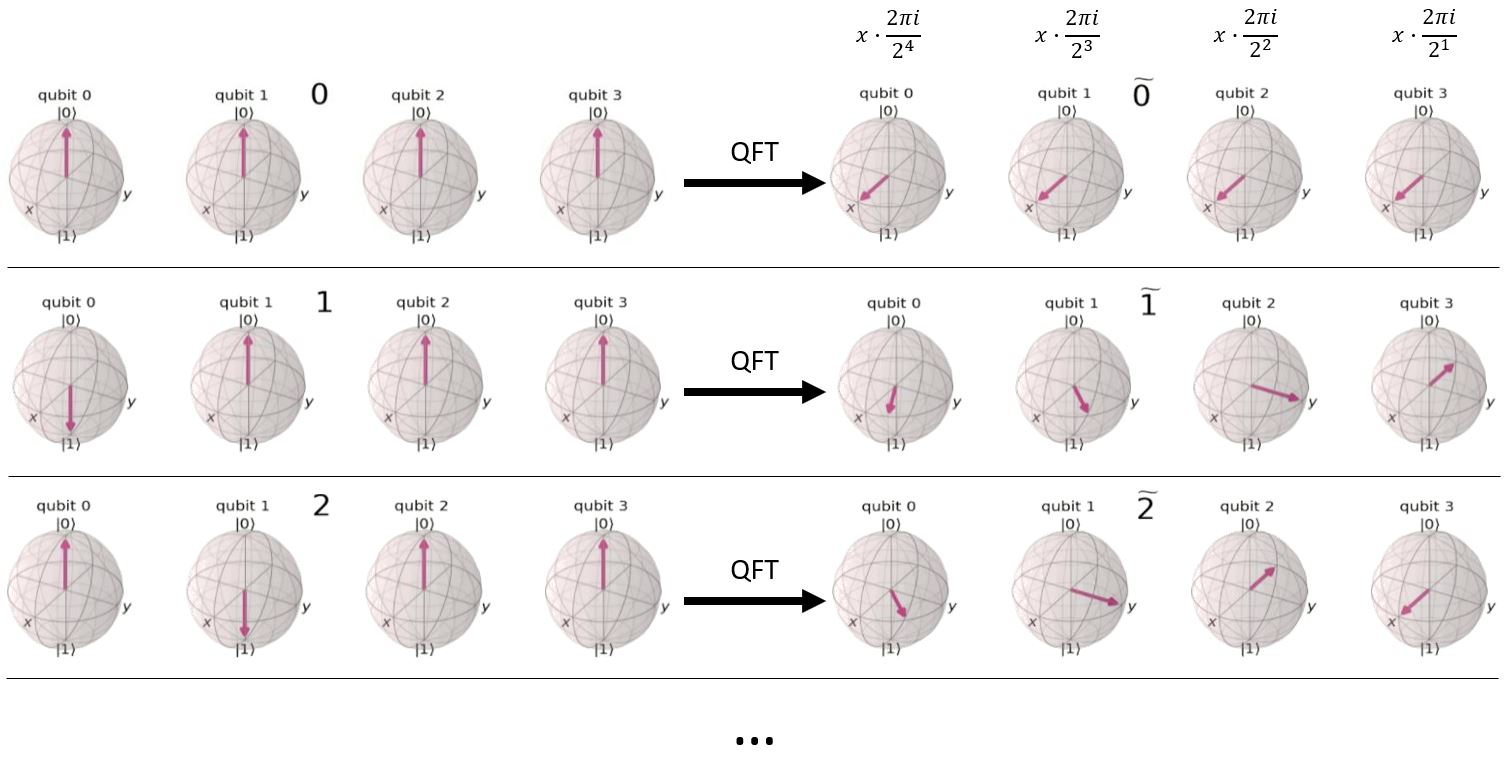
\includegraphics[width=100]{content/qft_example.JPG}
    \caption{Beispielhafte Darstellung einer Quantum Fourier Transformation mit vier Qubits und \(x_{dez} \in \{0,1,2,...\}, \quad max(x_{dez}) = 15\). (ANIS u. a., 2021, Vgl. Textbook ’Quantum Fourier Transform’ - Chapter 2)}


\end{figure}

\newline 
\exercise[type=multipleChoice]{
    \question{Frage: Was ist der Zweck einer QFT?}
    \possibleAnswers{
        \item 1) Die Messung von speziellen Zuständen.
        \item 2) Die Verschränkung von Qubits.
        \item 3) Die Transformation von Qubits in eine Fourier-Basis.
        \item 4) Mit einer QFT werden Störsignale entfernt.
        }
    \result{3}
}
\newline \newline

Um die QFT in der realen Welt anzuwenden, muss die vorherige Formel zu einem Quantum Circuit umgebaut werden. Hierfür werden zwei verschiedene Gates verwendet: H-Gates und Controlled-UROT-Gates. \newline

Ein CROT-Gate ist parametrisiert und besteht aus einem UROT-Gate (Unitary Rotation Gate):
\begin{equation}
    CROT_k=\begin{bmatrix}
        I & 0 \\ 0 & UROT_k
    \end{bmatrix}, \quad
    UROT_k = \begin{bmatrix}
        1 & 0 \\ 0 & \exp (\frac{2 \pi i}{2^k})
    \end{bmatrix}.
\end{equation}

\begin{figure}
    \centering
    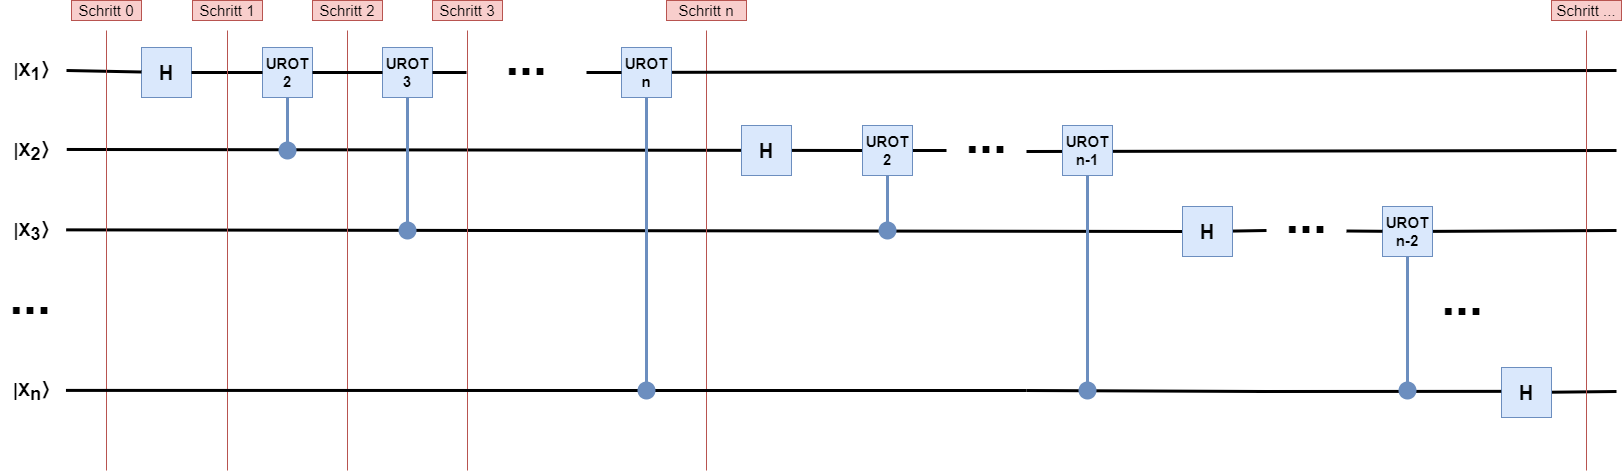
\includegraphics[width=100]{content/qft-circuit.png}
    \caption{Quantum Fourier Transformation Circuit mit \(n\) Qubits}
    \label{fig:qftCircuit}
\end{figure}


Die Anzahl an Gates pro Leitung nimmt linear mit der Rangfolge ab. Somit befinden sich auf der ersten Leitung \(n\) Gates
und auf der letzten nur noch eins. \newline
Jedes Qubit durchläuft zu Beginn ein H-Gate, was denselben Effekt wie eine UROT-Gate Rotation mit dem Parameter eins hat.
Die Größe der UROT-Gate Rotationen sind abhängig von der Anzahl der bereits durchgeführten UROT-Gates auf der jeweiligen Leitung.
Das heißt, dass der UROT-Gate Parameter \(k\) immer die Anzahl der bereits ausgeführten Gates auf der jeweiligen Leitung plus eins ist.
\newline
Im folgenden Beispiel wird der Zustand eines QFT-Circuits \(\Ket{\psi}\) mit drei Qubits in sechs Schritten Stück für Stück berechnet:


\begin{align*}
    \Ket{\psi_1} & = \frac{1}{\sqrt{2}}\begin{pmatrix}\Ket{0} + \exp{(x_1\cdot\frac{2\pi}{2})}\Ket{1}\end{pmatrix} \otimes \Ket{x_2} \otimes \Ket{x_3}
    \\
    \Ket{\psi_2} & =  \frac{1}{\sqrt{2}}\begin{pmatrix}\Ket{0} + \exp{(x_1\cdot\frac{2\pi}{2} + x_2\cdot\frac{2\pi}{4})}\Ket{1}\end{pmatrix} \otimes \Ket{x_2} \otimes \Ket{x_3}
    \\
    \Ket{\psi_3} & =  \frac{1}{\sqrt{2}}\begin{pmatrix}\Ket{0} + \exp{(x_1\cdot\frac{2\pi}{2} + x_2\cdot\frac{2\pi}{4} + x_3\cdot\frac{2\pi}{8})}\Ket{1}\end{pmatrix} \otimes \Ket{x_2} \otimes \Ket{x_3}                                                                            \\
    \Ket{\psi_4} & =  \frac{1}{\sqrt{2}}\begin{pmatrix}\Ket{0} + \exp{(x_1\cdot\frac{2\pi}{2} + x_2\cdot\frac{2\pi}{4} + x_3\cdot\frac{2\pi}{8})}\Ket{1}\end{pmatrix}  \otimes \begin{pmatrix}\Ket{0} + \exp{(x_2\cdot\frac{2\pi}{2})}\Ket{1}\end{pmatrix} \otimes \Ket{x_3}
    \\
    \Ket{\psi_5} & =  \frac{1}{\sqrt{2}}\begin{pmatrix}\Ket{0} + \exp{(x_1\cdot\frac{2\pi}{2} + x_2\cdot\frac{2\pi}{4} + x_3\cdot\frac{2\pi}{8})}\Ket{1}\end{pmatrix} \otimes                                                                                                        \\ & \frac{1}{\sqrt{2}}\begin{pmatrix}\Ket{0} + \exp{(x_2\cdot\frac{2\pi}{2} + x_3\cdot\frac{2\pi}{4})}\Ket{1}\end{pmatrix} \otimes \Ket{x_3}
    \\
    \Ket{\psi_6} & =  \frac{1}{\sqrt{2}}\begin{pmatrix}\Ket{0} + \exp{(x_1\cdot\frac{2\pi}{2} + x_2\cdot\frac{2\pi}{4} + x_3\cdot\frac{2\pi}{8})}\Ket{1}\end{pmatrix} \otimes                                                                                                        \\ & \frac{1}{\sqrt{2}}\begin{pmatrix}\Ket{0} + \exp{(x_2\cdot\frac{2\pi}{2} + x_3\cdot\frac{2\pi}{4})}\Ket{1}\end{pmatrix} \otimes \frac{1}{\sqrt{2}}\begin{pmatrix}\Ket{0} + \exp{(x_3\cdot\frac{2\pi}{2})}\Ket{1}\end{pmatrix}
\end{align*}


\newline \newline
\exercise[type=multipleChoice]{
    \question{Frage: Was ist äquivalent zu einem UROT-Gate mit dem Parameter \(1\)?}
    \possibleAnswers{
        \item 1) Ein H-Gate.
        \item 2) Ein H-Gate und ein Z-Gate.
        \item 3) Ein Controlled-Z Gate.
        \item 4) Ein Controlled-NOT Gate.
        }
    \result{1}
}

\newline \newline
\subsection{Quellen}
[ANIS u. a. 2021] Qiskit: An Open-source Framework for Quantum Computing. 2021\newline
[Nielsen und Chuang 2001] Nielsen, Michael A. ; Chuang, Isaac L.: Quantum computation and quantum information. In: Phys. Today 54 (2001), Nr. 2, S. 60\newline

